\documentclass{article}
\usepackage[english,russian]{babel}
\usepackage{amsmath}

%графика
\usepackage{wrapfig}
\usepackage{graphicx}
\usepackage{pgfplots}


%%% Работа с картинками
\usepackage{graphicx}  % Для вставки рисунков
\graphicspath{{images/}{images2/}}  % папки с картинками
\setlength\fboxsep{3pt} % Отступ рамки \fbox{} от рисунка
\setlength\fboxrule{1pt} % Толщина линий рамки \fbox{}
\usepackage{wrapfig} % Обтекание рисунков и таблиц текстом

 % для диаграмм
\usepackage{pgf}
\usepackage{tikz}
\usepackage[utf8]{inputenc}
\usetikzlibrary{arrows,automata}
\usetikzlibrary{positioning}
\tikzset{
    state/.style = {draw, rounded corners, 
                 minimum width=22mm, minimum height=5mm, align=center},
}


\usepackage{tcolorbox}

% Set page size and margins
% Replace `letterpaper' with `a4paper' for UK/EU standard size
\usepackage[letterpaper,top=2cm,bottom=2cm,left=3cm,right=3cm,marginparwidth=1.75cm]{geometry}

% Useful packages
\usepackage{amsmath}
\usepackage{amssymb}
\usepackage{graphicx}
\usepackage{fixltx2e}
\usepackage[colorlinks=true, allcolors=blue]{hyperref}
\usepackage{pgf}
\usepackage{array}
\newenvironment{conditions}
  {\par\vspace{\abovedisplayskip}\noindent\begin{tabular}{>{$}l<{$} @{${}={}$} l}}
  {\end{tabular}\par\vspace{\belowdisplayskip}}

\usepackage{geometry}
\geometry{left=25mm,right=25mm,
 top=25mm,bottom=25mm}

\title{Quantitative Analytics.\\
Lectures. Week 5. \\
Торговля опционами. 5 Лекция Антона Филатова}
\author{Михаил Сизов}

% Колонтитулы
\usepackage{fancyhdr}
\pagestyle{fancy}
\renewcommand{\headrulewidth}{0.1mm}  
\renewcommand{\footrulewidth}{0.1mm}
\lfoot{}
\rfoot{\thepage}
\cfoot{}
\rhead{CMF-2022}
\chead{}

\begin{document}
\maketitle

% Оглавление
\setcounter{tocdepth}{1} % {2} - в оглавлении участвуют chapter, section и subsection. {1} - только chapter и section
\renewcommand\contentsname{Contents}
\tableofcontents
\newpage

% \section{Dictionary, Definitions, Abbreviations}

% \subsection{Dictionary}
% \begin{itemize}
%     \item IR - Interest rate - процентная ставка.
%     \item Compounding - платежи (idk)
% \end{itemize}

% \subsection{Definitions and Abbreviations}
% \begin{itemize}
%     \item SAR - Stated annual rate.
%     \item EAR - Effective annual rate.
%     \item FoC - Frequency of Compounding
%     \item PMT - Payment
%     \item r - Interest rate (at the moment). 
% \end{itemize}

\renewcommand{\labelitemi}{\tiny$\bullet$}
\renewcommand{\figurename}{Fig.}

 
\section{Что такое Vega?}
\begin{center}  
Vega = $\frac{\partial MV}{\partial Volume}$ \\
\end{center}
Vega показывает насколько изменится стоимость актива, при изменится волатильность \\

\section{Что такое Delta Hedging? }
Рассмотрим следующий опцион:
\begin{itemize} 
\item{Опцион call USD-RUB}
\item{k (strike) = 70}
\item{N (номинал) = 100 m\$}
\item{Te (время до экспиоации) = 1 месяц}
\item{Spot = 70 рублей} 
\end{itemize}
Попробуем оценить стоимость опциона с помощью бинарного дерева (представим, что через 1 месяц стоимость доллора будет или 71 или 69 рублей):
% GRAPH
\begin{figure}[h]
\centering
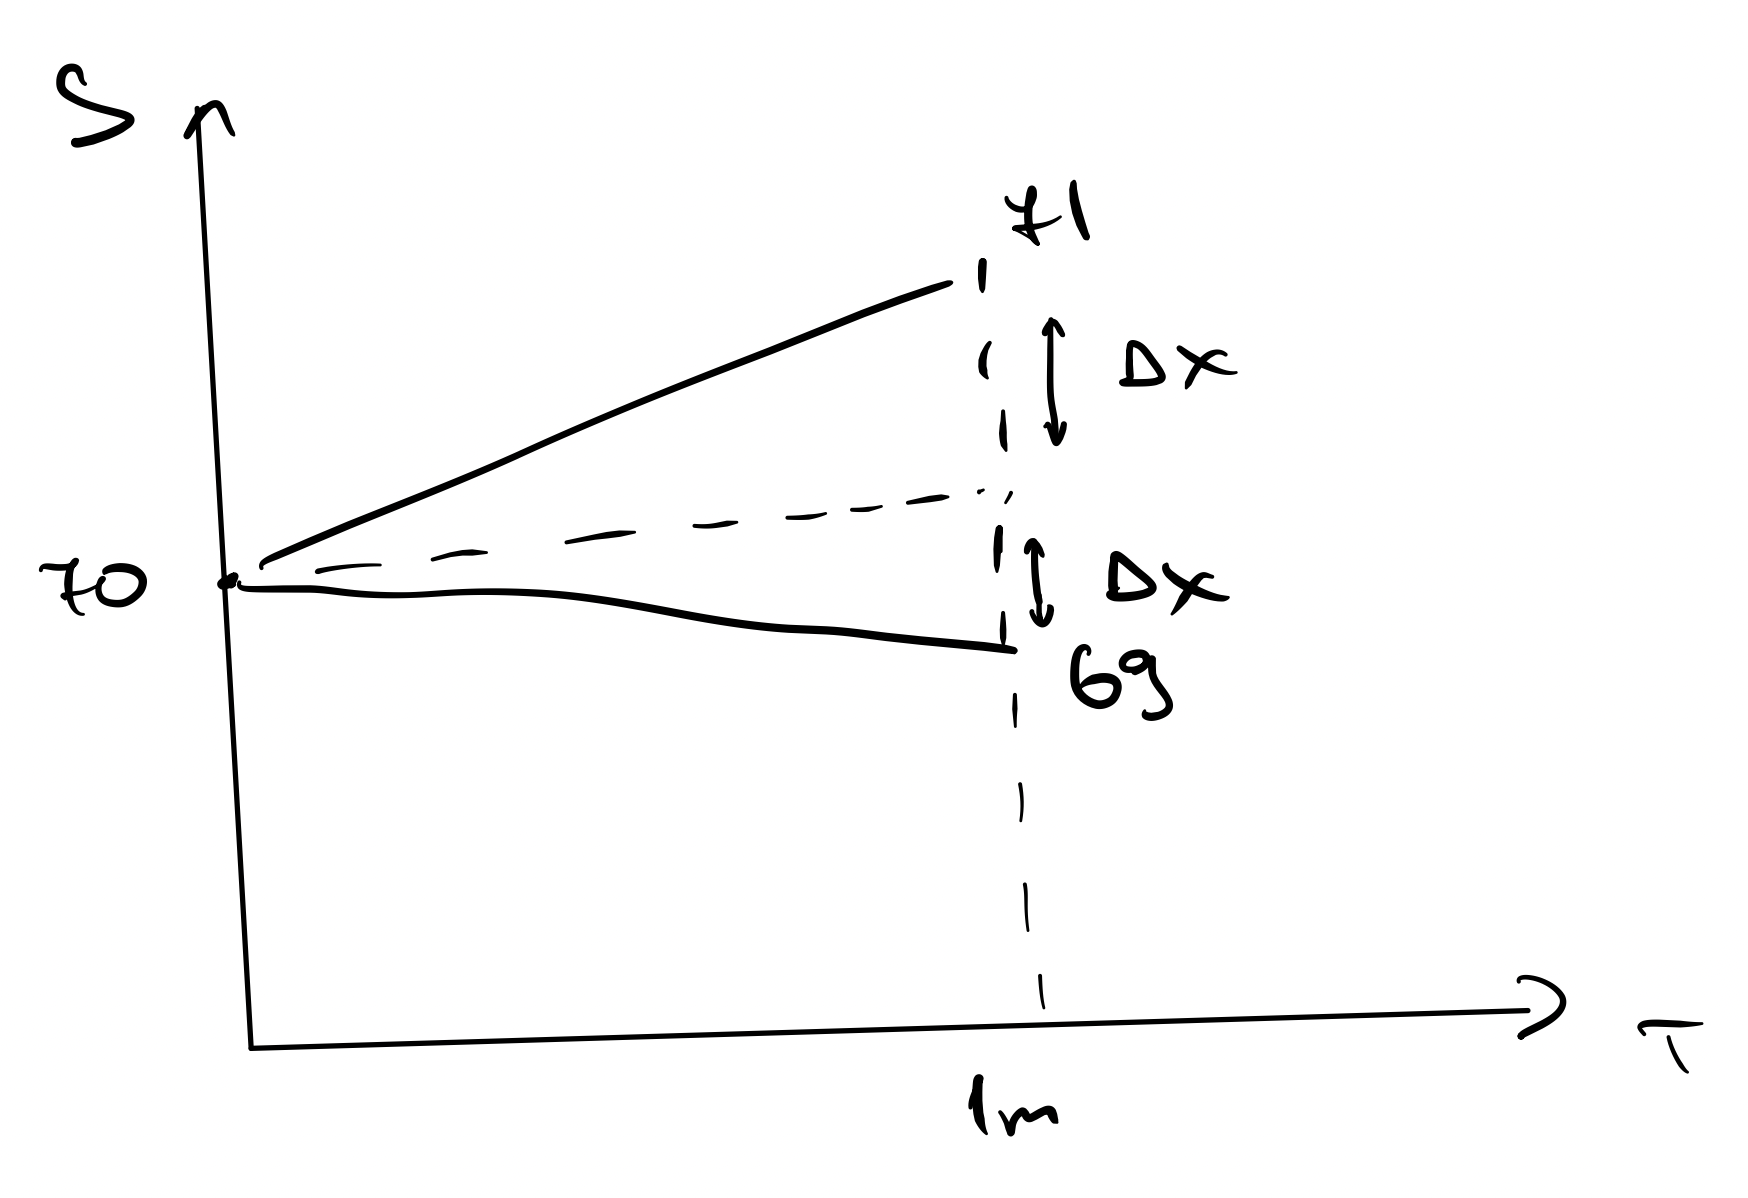
\includegraphics[width=0.8\linewidth]{Graph_1.png}
\caption{Потенциальная стоимость доллора на горизонте 1 месяц}
\label{fig:mpr}
\end{figure}
\\
Найдем стоимость опциона:
\\
M($T_{0}$ = 0) [стоимость опциона в 0 момент времени] \approx 0.5$\cdot$0 + 0.5$\cdot$100 млн рублей \\
Но выплата по опциону либо 0 либо 50 млн. Риски очень велики.\\\\
\textbf{Попробуем применить дельта хедж:} \\
Продаем 50 млн долларов  по 70 рублей. Рыночная стоимость скомбинированной позиции: \\
\begin{center}
    MV (рыночная стоимость) = 0.5$\cdot$(0 + 50) + 0.5$\cdot$(100- 50) = 50 млн руб 
\end{center}
MV (рыночная стоимость) не изменилась, но выплата стала фиксированной - 50 млн, вместо 100 млн или 0 с вероятностью 1/2. Таким образом мы уменьшаем риски. \\\\
\textbf{Основная задача хеджирования - лучше распредилить выплаты по разным событиям, чтобы ументьшить риски. \\
Идея дельта хеджирования - добавить такую позицию в базовый актив, чтобы чувствительность портфеля к стоимости базового актива стала 0.}
\\\\
Формула дельты: \\
\begin{center} 
Delta = $\frac{\partial MV}{\partial Spot}$ 
\end{center}
\\
Используется в вычислении методов, но в реальном трейдинге едва ли применяется - из-за сложностей вычисления.
\\\\
\textbf{Рассмотрим реальную позицию:} 
\begin{itemize} 
\item{длинная позиция 100 m\$ vs  RUB по курсу 70}
\item{Спот = 70, Базавая валюта - доллары} 
\end{itemize}
\\
Как сделать так чтобы не было чувствительности к USDRUB: \textbf{войти в аналогичную, но короткую позицию}. \\
Delta - кол-во базовой валюты, которое нужно купить или продать, чтобы закрыть чувствительность к базовой валюте. \\\\
\textbf{Зачем нам нужна дельта:} \\
1) Понимать, как закрыть позицию. \\
2) Легко считать P&L: \\
Если спот вырос на 7 копеек (0.1\% от спота) и Delta = 100 m\$ : \\
\begin{center} 
PnL = Delta * процент роста спота = 100 k \$ 
\end{center} 
\\\\
\textbf{Что такое Currency Pair (Валютная пара) и Quatation:}
\begin{itemize}
\item{Currency Pair (Валютная пара)  - например (USD - RUB, AUD - USD, etc.)}
\item{Quatation - как мы котируем валютную пару (может быть например AUD- USD, USD - AUD)} 
\end{itemize}

% \begin{tikzpicture}[->,>=stealth']

% \node (s1)  [state,text width=7cm] {\Large Risk-neutral approach};
% \node (s2)  [state,text width=7cm,  below=of s1]    
% {\Large Martingale property: \\ $\frac{V(t)}{D(t)} = E_t^{\mathbb{Q}}(\frac{V(T)}{D(T)} )$};

% \node (s3)  [state,text width=7cm,  below=of s2]    {\Large Equvivalent martingale properties};
% \node (s4)  [state,text width=7cm,  below=of s3]    {\Large Model for underlying using new measure };

% \node (s5)  [state,text width=7cm,  below=of s4]    {\Large Final payoff };


% \draw[->] (s1) to (s2);
% \draw[->] (s2) to (s3);
% \draw[->] (s3) to (s4);
% \draw[->] (s4) to (s5);


% \end{tikzpicture}
% \end{center}


%  \begin{itemize}

%      \item In the basic BSM economy, two assets are traded: a money market account $\beta$  and  a stock S - X(t).

%      \item The dynamics for $\beta$:
% \begin{center}   
%  $\frac{d \beta(t)}{\beta(t)}=r d t, \beta(0)=1$
%  \end{center}
%      \item The stock dynamics are assumed to satisfy GBMD:
% \begin{center}   
% $\frac{d S(t)}{S(t)}=\mu d t+\sigma d w(t)$
%  \end{center}
 
%     \item Deflated stock price:
% \begin{center}   
% $S^\beta(t)=\frac{S(t)}{\beta(t)}$
%  \end{center}
%      \item By Ito's lemma:
% \begin{center}   
% $\frac{d S^\beta(t)}{S^\beta(t)}=(\mu-r) d t+\sigma d W(t)$
% \end{center}

%      \item Applying Girsanov theorem:
% \begin{center}   
% $\frac{d \xi(t)}{\xi((t)}=-\theta d W(t), \theta=\frac{\mu-r}{\sigma}$
% \end{center}

%      \item Under new measure ${\mathbb{Q}}$ ,  $W^\beta(t)=W(t)+\theta t$
%     is a Brownian motion: 
     
% \begin{center}   
% $\frac{d S^\beta(t)}{S^\beta(t)}=\sigma W^\beta(t)$

% \\[0.3cm] $\frac{d S(t)}{S(t)}=r d t+\sigma W^\beta(t)$
% \end{center}

%      \item Hence stock dynamics:
% \begin{center}   
% $S(T)=S(t) e^{\left(r-\frac{1}{2} \sigma^2\right)(T-t)+\sigma\left(W^\beta(T)-W^\beta(t)\right)}$ , 
% $t \in[0, T]$
% \end{center}


%      \item Our final payoff depends on the final value of the underlying.

%      \item \textit{Discount bond} - paying at time T 1\$ for certain. \\ Application of basic derivative pricing equation immediately gives:
     
% \begin{center}   
% $P(t, T)=\beta(t) E_t^Q\left(\frac{1}{\beta(T)}\right)=E_t^Q\left(e^{-r(T-t)}\right)=e^{-r(T t)}$

% \end{center}


%      \item \textit{Europian call option} - paying $c(T) = (S(T) - K)^+$
% \begin{center}   
% $c(T)=e^{-r(T-t)} E_t^Q\left((S(T)-K)^{+}\right)$
% \\   [0.3cm]
% $c(t)=P(t, T) \int_{-\infty}^{+\infty}\left(S(t) e^{\left(r-\frac{1}{2} \sigma^2\right)(T-t)+z\sigma\sqrt{T-t}}-K\right)^{+} \varphi(z).$
% \end{center}

%      \item \underline{Theorem 2.1}: In the BS economy, the arbitrage-free time 1 price of the K-strike call-option maturing at time T is:
% \begin{center}   
% $c(T) = (S(T)N(d_1) - KP(t,T)N(d_2)$
% \\   [0.3cm]


% $ d_1_,_2 = \frac{ln(S(t)/K +(r \pm \sigma^2/2) (T-t)}{\sigma\sqrt{T-t}}$

%         where N(.) is a Gaussian cumulative distribution function:
%         $N(d)=\frac{1}{\sqrt{2 \pi}} \int_{-\infty}^d e^{-\frac{x^2}{2}} d x$ 
% \end{center}

%      \item \underline{Lemma 2.2}: In BS notation the following results holds:

% \begin{center}   
% $SN'(d_1)=Ke^{-r(T-t)}N'(d_2)$
% \end{center}

%         \textit{Proof}: recall that $d_2 = d_1 - \sigma \sqrt{T-t}$  and open brackets in the exponent.

















% \end{itemize}

% \section{Greeks}
%      \item Greeks to derive:
%           \\[0.3cm]  - Delta ($\Delta$) - sensitivity of option price to underlying price.
%           \\[0.3cm]   - Gamma ($\Gamma$) - sensitivity to option delta to underlying price.
%           \\[0.3cm]   - Vega ($\vartheta$) - sensitivity of option price to volatility.



% \begin{center}   
% $\Delta=\frac{\partial C}{\partial S}=N\left(d_1\right)+S \frac{\partial N\left(d_1\right)}{\partial d_1} \frac{\partial d_1}{\partial S}-K P\left(t_1 T\right) \frac{\partial N\left(d_2\right)}{\partial d_2} \frac{\partial d_2}{\partial S}=$
% \\[0.2cm]
% $=N\left(d_1\right)+S N^{\prime}\left(d_1\right)\left[\frac{\partial d_1}{\partial S}-\frac{\partial d_2}{\partial S}\right]=N\left(d_1\right)$
% \end{center}


%         \\[0.3cm]   Note that: $N(d)=\frac{1}{\sqrt{2 \pi}} \int_{-\infty}^d e^{-\frac{x^2}{2}} d x$ ,  
%         $N^{\prime}(d)=\frac{1}{\sqrt{2 \pi}} e^{-\frac{d^2}{2}}$,    
%         $\frac{\partial d_1}{\partial S}=\frac{\partial d_2}{\partial S}$,  
%         $\quad S \frac{\partial N\left(d_1\right)}{\partial d_1}=K P(t, T)\frac{\partial N\left(d_2\right)}{\partial d_2}$





% \begin{center}   
% $\Gamma =\frac{\partial^2 C}{\partial S^2}=\frac{\partial}{\partial S} \frac{\partial C}{\partial S}=\frac{\partial}{\partial S} N\left(d_1\right)=\frac{\partial N\left(d_1\right)}{\partial d_1} \frac{\partial d_1}{\partial S} =N^{\prime}\left(d_1\right) \cdot \frac{1}{S \sigma \sqrt{T-t}}$
% \end{center}

%         \\[0.3cm]   Note that: $\frac{\partial d_1}{\partial S}=\frac{1}{S \partial \sqrt{T-t}}$
%         \\[0.1cm]
        
% \begin{center}   
% $\vartheta=\frac{\partial C}{\partial \sigma}=S \frac{\partial N\left(d_1\right)}{\partial d_1} \frac{\partial d_1}{\partial \sigma}-K P(t, T) \frac{\partial N(d_2)}{\partial d_2} \frac{\partial d_2}{\partial \sigma} =S \frac{\partial N\left(d_1\right)}{\partial d_1}\left[\frac{\partial d_1}{\partial \sigma}-\frac{\partial d_1}{\partial \sigma}\right]=S \frac{\partial N\left(d_1\right)}{\partial d_1} \sqrt{T-t}$
% \end{center}
     
%         \\[0.3cm]       Note that: $\quad S \frac{\partial N\left(d_1\right)}{\partial d_1}=K P(t, T)\frac{\partial N\left(d_2\right)}{\partial d_2}$ - lemma 2.2  again and $\quad d_2=d_1-\sigma \sqrt{T-t}$.




\end{document}
